\section{Introduction}\label{sec:introduction}

% Multi-Agent PathFinding or MAPF \cite{ststfekomawaliatcokubabo19a,ststfekomawaliatcokubabo19b,stern19a} for short, is a fundamental AI problem that has a wide-range real application: GPS, video-games, routing, planning, traffic control etc. In few words, consider agents moving in an environment, going from an initial to a goal position; MAPF is about finding a path for each agent, such as there is no collision between them. Multiple approaches exist; Search-algorithm (CBS \cite{shstfest15a}) or reduction solving based (\cite{barsva19a}). 
% In this report we focus on an approach call ``Plan Merging'', this approach aims to solve MAPF problems by using two distinct steps; computing a set of paths for each agent independently (which correspond to classic pathfinding / single-agent pathfinding~\cite{foghkuhagu21a}). We will refer to this step as Individual Path Finding. The second step, to find a solution avoiding collision using the previously computed paths. Formalization of each step will be described in their respective sections. The interest in this approach is due to pathfinding complexity which is lower than MAPF complexity \cite{nebel19a}; the idea is then to use this property to expect saving computation time or space complexity. Plan Merging is based on conflict; the idea is to determine which are the interesting paths to merge using conflicts. Conflict are expressed in two forms, potential conflict and heatmap.
% The approach in its definition is close to CBS, however, the planning part of CBS stops if a conflict occurs and re-iter the planning part considering the conflict previously encountered which is not the case for  Individual Path Finding; the conflict handling would be in the merging section.


Multi-Agent Pathfinding (MAPF)~\cite{ststfekomawaliatcokubabo19a,ststfekomawaliatcokubabo19b,stern19a}, is an artificial Intelligence problem with diverse real-world applications such as warehouse management~\cite{wurman2008coordinating}, video games~\cite{ma2017feasibility}, routing, planning, and robotics~\cite{veloso2015cobots}. In essence, MAPF involves multiple agents moving within an environment, aiming to navigate from initial positions to goal locations. The primary challenge in MAPF is to find individual paths for each agent, ensuring that they do not collide. Various techniques have been developed to tackle this problem, including search algorithms like CBS~\cite{shstfest15a} (Conflict-Based Search) and reduction-based-solving methods~\cite{barsva19a}.

In this Master Thesis, we focus on the "Plan Merging" approach, which aims to solve MAPF problems through a three-steps process. The first step, denoted as Individual Path Finding, involves computing paths for each agent independently, which corresponds to classic pathfinding or single-agent pathfinding~\cite{foghkuhagu21a}. The second step denoted Path Selection focuses on finding a collision-free solution using the previously computed path where selection occurs using conflict represented in two ways; potential conflict and likelihood of presence using heatmaps. The third and last step of Plan Merging is to find a solution, by 1), reducing the size of the problem using paths selected in previous step to delimitate a subgraph. Or by 2), using the conflict-free paths issued from previous step as a baseline for a MAPF algorithm. The appeal of this approach lies in the lower complexity of pathfinding compared to the overall MAPF problem~\cite{nebel19a}. The Plan Merging approach anticipates saving computation time at the cost of a possible loss of optimality. For instance, given some robots in a warehouse moving from a shelf to another, we first computes some paths for them regardless of their conflict among each other. We then eliminate paths that are ``bad'' through a heuristic, which can be in our case, through heatmap. A heatmap being a representation of potential conflict among paths achieved by allocating a value from 0 to 1 for each vertex. The value representing the likelihood of having a conflict. If a complete conflict-free solution cannot be found among the remaining paths, we use the paths that are not conflicting as a preprocessing step for a classical MAPF approach. The following figure shows an example with three agents. In this example, a solution is directly found by eliminating the right paths. 

\begin{figure}[H]
    \centering
    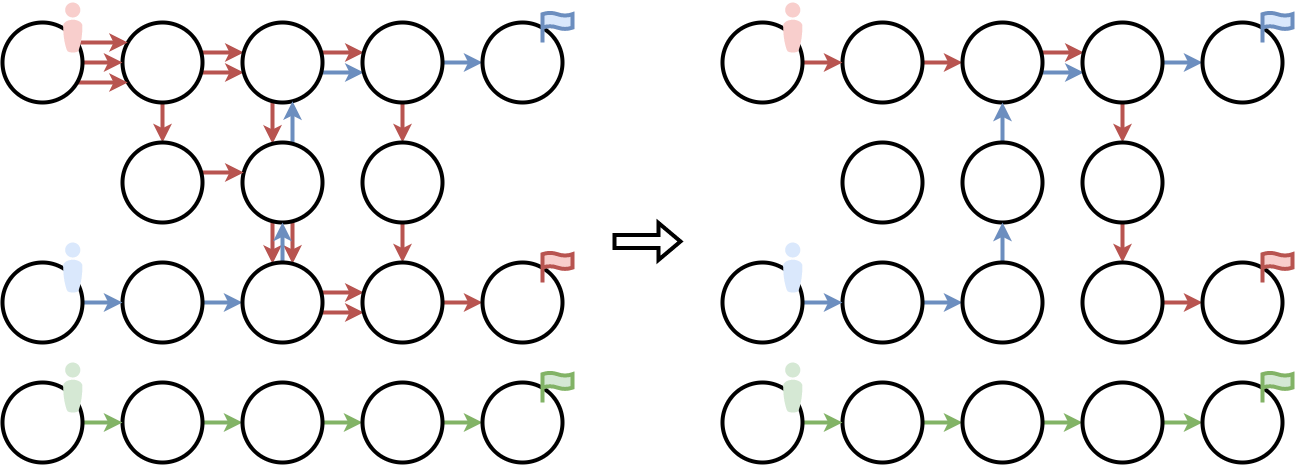
\includegraphics[width=9cm]{img/pm_example_intro.png}
\end{figure}

The approach in its definition is inspired and close to CBS's definition, however, the planning part of CBS stops if a conflict occurs and compute another time the planning part considering the conflict previously encountered, which is not the case for the Individual Path Finding; conflicts are handled after Individual Path Finding. 

Furthermore, our study shows that in certain cases, especially for large instances, our proposed approaches can outperform classical MAPF methods in terms of computation time. On the other hand, the results  outline the limits of the Plan Merging techniques we have developed. In certain scenarios, obtaining a complete solution might prove challenging or not feasible with the approaches we introduced, indicating the need to recognize the inherent limitations of the Plan Merging strategies.